\documentclass[11pt]{article}
\usepackage[margin=1in]{geometry}
\usepackage{amsmath,amssymb,amsthm,mathtools}
\usepackage{graphicx}
\usepackage{hyperref}

\newtheorem{theorem}{Theorem}
\newtheorem{remark}{Remark}
\newcommand{\E}{\mathbb E}
\newcommand{\cube}{\{-1,1\}^n}
\newcommand{\wh}{\widehat}

\title{Sharp heat smoothing for sign-aligned Walsh spectra}
\author{Autonomous solution packet for arXiv:1406.7855}
\date{August 11, 2026}

\begin{document}
\maketitle

\begin{center}
\fbox{\parbox{0.91\textwidth}{
\textbf{Status: candidate partial result, likely valid.}
For every even $p$ and for $p=\infty$, the full heat-smoothing estimate
holds with sharp constant one on a translation-invariant cone of tail
functions.  The unrestricted scalar conjecture remains open.
}}
\end{center}

\section{The conjecture and the coefficient cone}

On the discrete cube with uniform probability measure, write
\[
 f=\sum_{S\subseteq[n]}\wh f(S)W_S,\qquad
 W_S(x)=\prod_{i\in S}x_i,
\]
and let
\[
 P_tf=\sum_Se^{-t|S|}\wh f(S)W_S,\qquad
 Lf=\sum_S|S|\wh f(S)W_S.
\]
The $k$-th tail space consists of functions for which
$\wh f(S)=0$ whenever $|S|<k$.  The Mendel--Naor heat-smoothing
conjecture asks whether, for every $1<p<\infty$, there is $c_p>0$ such
that
\[
 \|P_tf\|_p\le e^{-c_pkt}\|f\|_p                              \tag{HS}
\]
for every dimension, tail degree, and scalar tail function.

\begin{quote}
A real function $f$ has a \emph{sign-aligned Walsh spectrum} if there
exist $\varepsilon\in\{-1,1\}$ and
$\tau\in\{-1,1\}^n$ such that
\[
 \varepsilon W_S(\tau)\wh f(S)\ge0\qquad(S\subseteq[n]).
                                                                    \tag{SA}
\]
\end{quote}
The condition is invariant under cube translations and overall sign.
It imposes no upper bound on the Fourier degrees and therefore differs
from the narrow-spectrum hypotheses treated in later work.

\begin{theorem}[sharp even-moment heat smoothing]\label{thm:main}
Let $k\ge1$, let $f:\cube\to\mathbb R$ belong to the $k$-th tail space,
and suppose that $f$ satisfies\/ {\rm(SA)}.  Then, for every integer
$m\ge1$ and every $t\ge0$,
\[
 \|P_tf\|_{2m}\le e^{-kt}\|f\|_{2m}.                            \tag{1}
\]
The same estimate holds for $p=\infty$.  The rate is sharp.
\end{theorem}

\section{The zero-symmetric-difference expansion}

The proof rests on the following elementary lemma.

\begin{theorem}[positive-coefficient coercivity]\label{thm:coercive}
Suppose
\[
 g=\sum_{\substack{S\subseteq[n]\\|S|\ge k}}b_SW_S,
 \qquad b_S\ge0.
\]
Then, for every integer $m\ge1$,
\[
 \E\big[g^{2m-1}Lg\big]\ge k\,\E[g^{2m}].                      \tag{2}
\]
\end{theorem}

\begin{proof}
Orthogonality of the Walsh characters, together with
$W_{S_1}\cdots W_{S_r}=W_{S_1\triangle\cdots\triangle S_r}$,
gives
\[
 \E[g^{2m}]
 =
 \sum_{\substack{S_1,\ldots,S_{2m}\\
 S_1\triangle\cdots\triangle S_{2m}=\varnothing}}
 \prod_{j=1}^{2m}b_{S_j}.                                     \tag{3}
\]
Similarly,
\[
 \E[g^{2m-1}Lg]
 =
 \sum_{\substack{S_1,\ldots,S_{2m}\\
 S_1\triangle\cdots\triangle S_{2m}=\varnothing}}
 |S_{2m}|\prod_{j=1}^{2m}b_{S_j}.                             \tag{4}
\]
The index set and coefficient product in (4) are invariant under every
permutation of the $2m$ positions.  Averaging the distinguished degree
over all positions therefore rewrites (4) as
\[
 \frac1{2m}
 \sum_{\substack{S_1,\ldots,S_{2m}\\
 S_1\triangle\cdots\triangle S_{2m}=\varnothing}}
 \left(\sum_{j=1}^{2m}|S_j|\right)
 \prod_{j=1}^{2m}b_{S_j}.                                     \tag{5}
\]
Every nonzero product in (5) has $|S_j|\ge k$ for all $j$, and every
product is nonnegative.  Thus (5) is at least $k$ times (3).
\end{proof}

\section{Proof of Theorem \ref{thm:main}}

\begin{proof}
Translations $f(x)\mapsto f(\tau x)$ and multiplication by an overall
sign preserve every $L_p$ norm and commute with $P_t$ and $L$.
We may therefore assume $\wh f(S)\ge0$ for every $S$.

Put $g_t=P_tf$.  Its Walsh coefficients
$e^{-t|S|}\wh f(S)$ remain nonnegative and remain supported on degrees
at least $k$.  Differentiating the finite sum and applying Theorem
\ref{thm:coercive} gives
\begin{align*}
 \frac{d}{dt}\E[g_t^{2m}]
 &=-2m\,\E[g_t^{2m-1}Lg_t]\\
 &\le-2mk\,\E[g_t^{2m}].
\end{align*}
Gronwall's inequality yields
$\E[(P_tf)^{2m}]\le e^{-2mkt}\E[f^{2m}]$, which is (1).

For the endpoint, nonnegativity of the coefficients shows
\[
 \|f\|_\infty=\sum_S\wh f(S):
\]
the triangle inequality gives the upper bound and equality is attained
at the all-ones point.  Consequently
\[
 \|P_tf\|_\infty
 =\sum_Se^{-t|S|}\wh f(S)
 \le e^{-kt}\sum_S\wh f(S)
 =e^{-kt}\|f\|_\infty.
\]
Finally, a single Walsh character $W_S$ with $|S|=k$ gives equality for
every $p$, proving sharpness.
\end{proof}

\section{Scope and obstruction to a full result}

For arbitrary real coefficients, formulas (3)--(5) remain true but their
products can have both signs.  The termwise degree comparison then fails:
the general conjecture is exactly asking for a way to control those
cancellations in a nonlinear $L_p$ pairing.

Replacing the coefficients by their absolute values produces a
sign-aligned majorant, but the Walsh basis has no applicable
dimension-free unconditional estimate that compares its norm with the
original function.  Interpolation between adjacent even moments also has
the initial norms in the wrong direction.  Thus this argument does not
resolve non-even $p$ or unrestricted coefficient signs.

The source paper proves the degree-one case for all $p$ and the
arbitrary-degree case for three-valued functions.  Subsequent work gives
narrow-spectrum and holomorphic special cases, while still describing the
unrestricted scalar cube conjecture as open.  Targeted searches found no
matching sign-aligned even-moment theorem, but the novelty search was not
exhaustive.

The accompanying script \texttt{code/verify\_even\_moment.py} enumerates a
small cube and checks (2) for random nonnegative coefficients at $p=4$.
It is a numerical sanity check only.

\begin{thebibliography}{9}
\bibitem{HMO}
S. Heilman, E. Mossel, and K. Oleszkiewicz,
\emph{Strong contraction and influences in tail spaces},
arXiv:1406.7855; Trans. Amer. Math. Soc. 369 (2017), 4843--4863.

\bibitem{EI}
A. Eskenazis and P. Ivanisvili,
\emph{Polynomial inequalities on the Hamming cube},
arXiv:1902.02406.

\bibitem{IN}
P. Ivanisvili and F. Nazarov,
\emph{On Weissler's conjecture on the Hamming cube I},
arXiv:1907.11359.

\bibitem{Z}
H. Zhang,
\emph{Heat-smoothing for holomorphic subalgebras of free group von
Neumann algebras},
arXiv:2205.12833.
\end{thebibliography}

\clearpage
\section*{Source context}

Page 1 of the locally rendered arXiv:1406.7855 source states the full
heat-smoothing conjecture.  The abstract also records which influence
questions are answered in the same paper.

\begin{center}
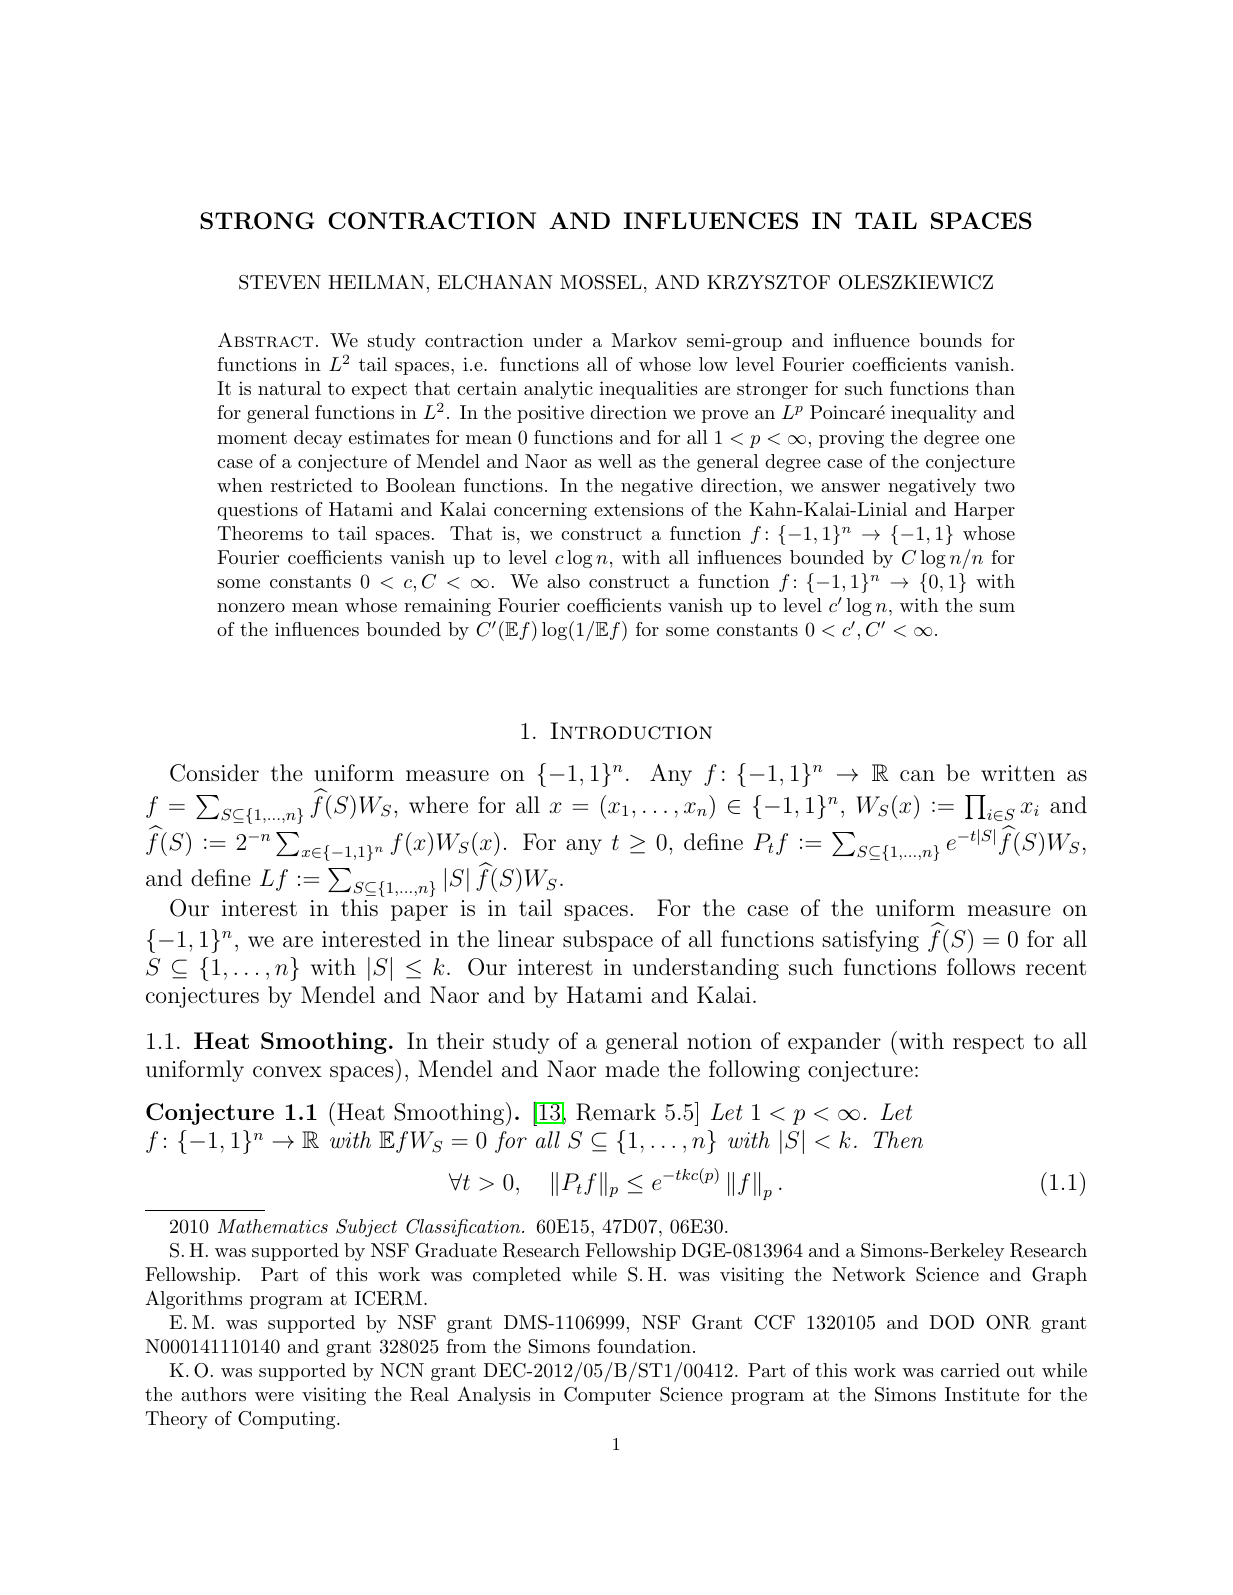
\includegraphics[width=0.76\textwidth]{figures/source_conjecture_page.png}
\end{center}

\end{document}
